\section{Preliminaries, Definitions}\label{sec:prelims}

We begin by introducing the necessary definitions and terminology, as
well as a few observations about the mathematical objects of interest
which will be of use later.  We carefully lay out these definitions so
as to align with an intuitive understanding of the concepts and to
appease the astute reader who may be concerned with edge cases,
geometric weirdness, and nonmeasurability.

\begin{definition}
  A \textbf{region} $\Omega$ in $\mathbb{S}^2$ or 
  in $\R^2$ is an non-empty open set together with its
  boundary such that the region is measurable, its boundary is
  measurable, and it is connected.
\end{definition}

We choose this definition so that concepts of the `area' and
`perimeter' of a region are well-defined concepts.  Throughout, we
restrict our attention to the plane $\mathbb{R}^2$ 
and the surface of the unit sphere $\mathbb{S}^2$ equipped
with the standard measures and metrics.  We leave the consideration of
other surfaces, measures, and metrics to future work.

\begin{definition}
	In a metric space, a \textbf{geodesic} between two points is the shortest path connecting them with respect to the metric.
	In the plane, geodesics are line segments, and on the surface of the sphere, geodesics are segments of great circles.
\end{definition}

\begin{definition}
  A \textbf{compactness score function} $\mathcal{C}$ is a function from
  the set of all regions to the positive real numbers.  We adopt the
  convention that a region with a \textit{higher} compactness score is
  \textit{more} compact, and this naturally induces a partial order over
  the set of all regions, where $A$ is at least as compact as $B$ if and
  only if $\mathcal{C}(A)\geq \mathcal{C}(B)$.
\end{definition}

The final major definition we need is that of a \textit{map
projection}.  In reality, the regions we are interested in comparing
sit on the surface of the Earth (i.e. a sphere), but these regions are
often examined as being projected onto a flat sheet of paper or
computer screen, and which means that the regions drawn in any flat
map object are subject to such a projection.

\begin{definition}
  A \textbf{map projection} $\varphi$ is a locally defined 
  diffeomorphism from a region on the sphere to a region on the 
  plane. 
\end{definition}

Intuitively, a map projection is a well-defined, invertible function between the sphere and the plane which sends regions on the sphere to regions in the plane.

\begin{definition}
  We use the word \textbf{transformation} [of the plane/sphere] to mean
  to a diffeomorphism from the plane or sphere to itself.
\end{definition}

Since the image of a region under a map projection $\varphi$ is also
a region, we can examine the compactness score of that region both 
before and after applying $\varphi$, and this is the heart of the
problem we address in this paper.  We demonstrate, for several
standard choices of compactness scores $\mathcal{C}$, that the order
induced by $\mathcal{C}$ is different than the order induced by
$\mathcal{C}\circ\varphi$ for \textit{any} choice of map projection
$\varphi$.

\begin{definition}
  We say that a map projection $\vphi$ \textbf{preserves the  
  compactness score ordering} of a score $\mc{C}$ if for any regions 
  $\Omega,\Omega'$ in the sphere, $\mc{C}(\Omega)\ge \mc{C}(\Omega')$ 
  if and only if $\mc{C}(\vphi(\Omega)) \ge \mc{C}(\vphi(\Omega'))$ in the plane.
\end{definition}

  We observe that this is a weaker condition than simply preserving the raw compactness scores.  Additionally, $\vphi$ preserves a compactness score $\mc{C}$ 
  if and only if $\vphi^{-1}$ does.

\begin{definition}
  Let $\mbb{S}^2\subset \R^3$ be the unit sphere. A 
  \textbf{cap} on the sphere is a region of the 
  form $\kappa(h) = \{(x,y,z)\in \mbb{S}^2: z\ge h\}$.
\end{definition}

\begin{figure}
  \centering
  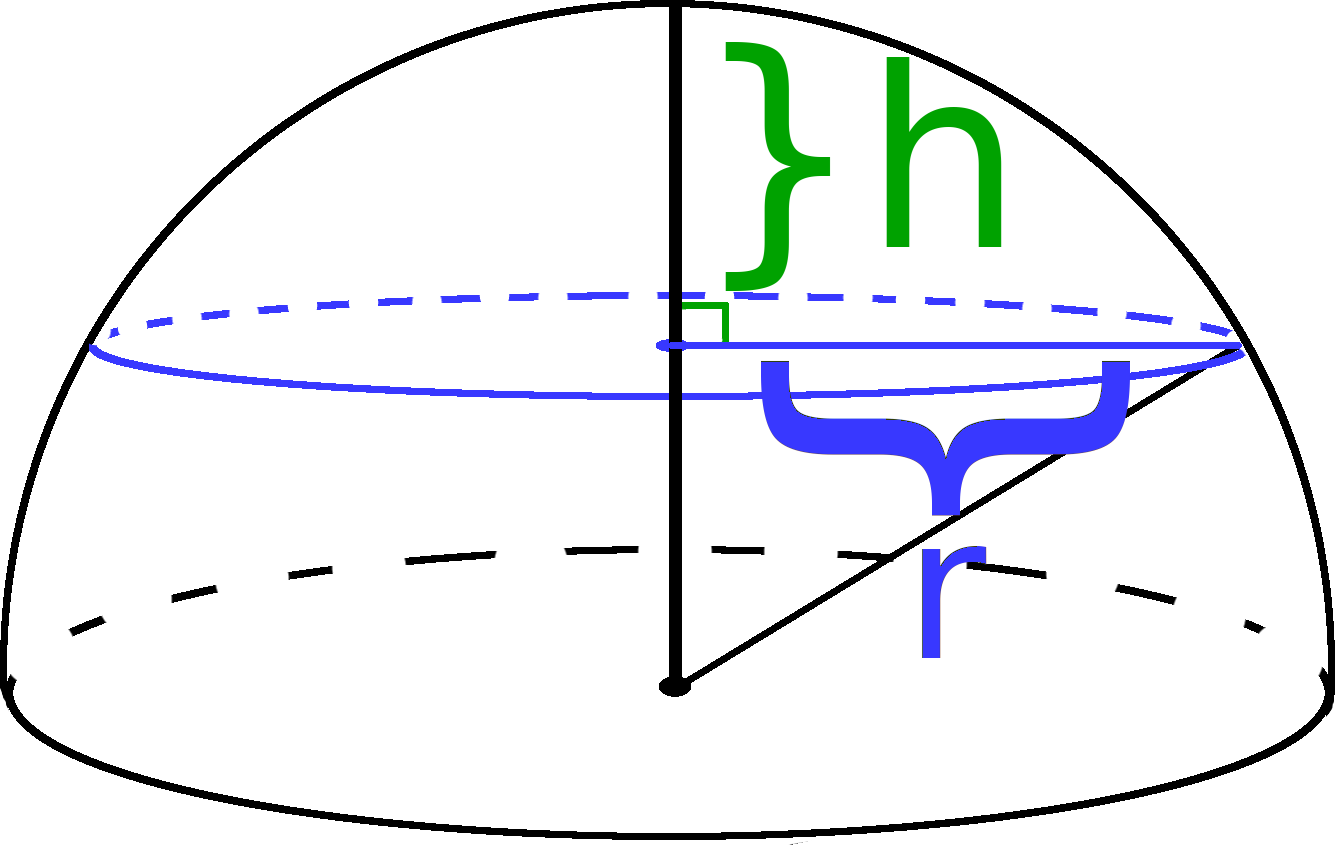
\includegraphics[width=.3\textwidth]{figs/spherecapschema}\\[1.5em]
  \caption{ The height and radius of a spherical cap. }
  \label{fig:caphr}
\end{figure}
